\section{lg\-Empty Class Reference}
\label{classlgEmpty}\index{lgEmpty@{lgEmpty}}
empty note based on {\bf lg\-Note} see GUIDO spec for description  


{\tt \#include $<$lgempty.h$>$}

Inheritance diagram for lg\-Empty::\begin{figure}[H]
\begin{center}
\leavevmode
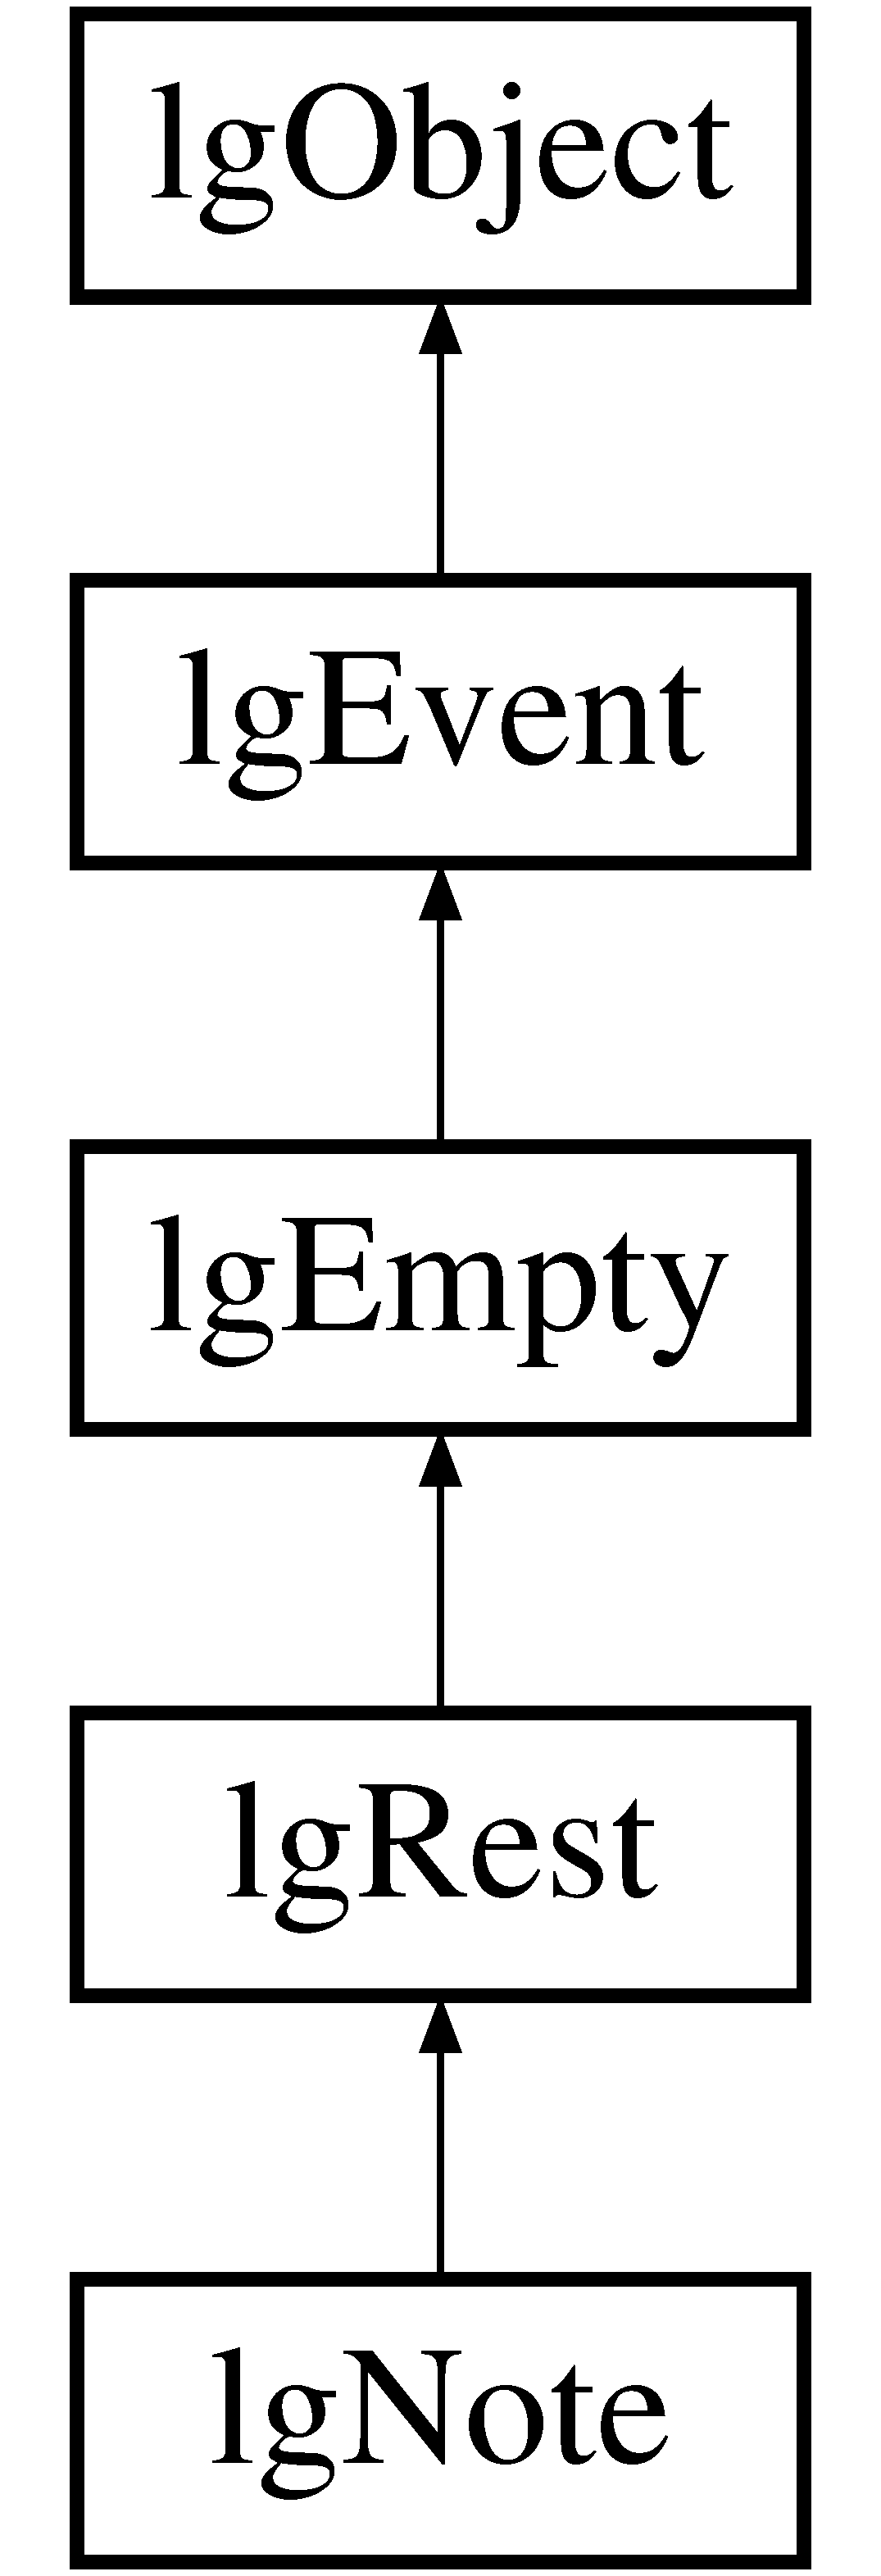
\includegraphics[height=5cm]{classlgEmpty}
\end{center}
\end{figure}
\subsection*{Public Member Functions}
\begin{CompactItemize}
\item 
virtual string {\bf to\-String} ({\bf lg\-Voice} $\ast$calling\-Seq=NULL)
\begin{CompactList}\small\item\em write \char`\"{}empty\char`\"{} \item\end{CompactList}\item 
{\bf lg\-Empty} (long int dur\-Num, long int dur\-Denom, int cdots, long int pos\-Num, long int pos\-Denom)
\end{CompactItemize}


\subsection{Detailed Description}
empty note based on {\bf lg\-Note} see GUIDO spec for description 



\subsection{Constructor \& Destructor Documentation}
\index{lgEmpty@{lg\-Empty}!lgEmpty@{lgEmpty}}
\index{lgEmpty@{lgEmpty}!lgEmpty@{lg\-Empty}}
\subsubsection{\setlength{\rightskip}{0pt plus 5cm}lg\-Empty::lg\-Empty (long int {\em dur\-Num}, long int {\em dur\-Denom}, int {\em cdots}, long int {\em pos\-Num}, long int {\em pos\-Denom})}\label{classlgEmpty_a1}




\subsection{Member Function Documentation}
\index{lgEmpty@{lg\-Empty}!toString@{toString}}
\index{toString@{toString}!lgEmpty@{lg\-Empty}}
\subsubsection{\setlength{\rightskip}{0pt plus 5cm}string lg\-Empty::to\-String ({\bf lg\-Voice} $\ast$ {\em calling\-Seq} = NULL)\hspace{0.3cm}{\tt  [virtual]}}\label{classlgEmpty_a0}


write \char`\"{}empty\char`\"{} 



Reimplemented from {\bf lg\-Event} {\rm (p.\,\pageref{classlgEvent_a1})}.

Reimplemented in {\bf lg\-Note} {\rm (p.\,\pageref{classlgNote_a0})}, and {\bf lg\-Rest} {\rm (p.\,\pageref{classlgRest_a0})}.

The documentation for this class was generated from the following files:\begin{CompactItemize}
\item 
{\bf lgempty.h}\item 
{\bf lgempty.cpp}\end{CompactItemize}
